\section{Die miese Gegenwart}

\subsection{Übersicht}

\tikzset{
	arrow/.style={
		->,
		thick,
		shorten >=0.4ex,
	},
}

\def\zugartText#1#2{%
	#1 - #2
}

\def\rowset{1ex}
\def\colset{2.2em}

\def\jezus#1{%
	\tiny\only<#1>{\color{red}\scriptsize}
}

\def\lowlife#1{
	\begin{figure}
		\begin{subfigure}{0.48\textwidth}
			\includegraphics[width=\textwidth]{gegenwart/#1-1}
		\end{subfigure}
		\hfill
		\begin{subfigure}{0.48\textwidth}
			\includegraphics[width=\textwidth]{gegenwart/#1-2}
		\end{subfigure}
	\end{figure}
}

\begin{frame}
	\frametitle{Zugarten}
	\begin{tikzpicture}
		{\jezus{2-6}
			\node[anchor=west] at (0.5*\colset, 0) (NV) {Nahverkehr};
			\draw [arrow](0,0) -- (NV.west);
		}
		{\jezus{7-9}
			\node [below=\rowset of NV.south] (FV) {Fernverkehr};
			\draw [arrow](0,0) -- (FV.west);
		}
		{\jezus{2-4}
			\node [anchor=west, right=\colset of NV.east] (SNV) {städtischen Raum};
			\draw [arrow] (NV.east) -- (SNV.west);
		}
		{\jezus{2}
			\node [anchor=west, right=\colset of SNV.east] (S1) {Straßenbahn};
			\draw [arrow] (SNV.east) -- (S1.west);
		}
		{\jezus{3}
			\node [below right=\rowset and 0cm of S1.south west] (S2) {U-Bahn};
			\draw [arrow] (SNV.east) -- (S2.west);
		}
		{\jezus{4}
			\node [below right=\rowset and 0cm of S2.south west] (S3) {S-Bahn};
			\draw [arrow] (SNV.east) -- (S3.west);
		}
		{\jezus{5}
			\node[anchor=west, below right=\rowset and 0 of SNV.south west](1) {\zugartText{RB}{Regionalbahn}};
			\draw [arrow] (NV.east) -- (1.west);
		}
		
		{\jezus{6}
			\node[below right=\rowset and 0cm of 1.south west] (2) {\zugartText{RE}{Regional-Express}};
			\draw [arrow] (NV.east) -- (2.west);
		}

		{\jezus{7}
			\node[below right=\rowset and 0cm of 2.south west] (3) {\zugartText{IC}{Intercity}};
			\draw [arrow] (FV.east) -- (3.west);
		}
		{\jezus{8}
			\node[below right=\rowset and 0cm of 3.south west] (4) {\zugartText{RE}{Eurocity}};
			\draw [arrow] (FV.east) -- (4.west);
		}
		{\jezus{9}
			\node[below right=\rowset and 0cm of 4.south west] (5) {\zugartText{RE}{Intercity-Express}};
			\draw [arrow] (FV.east) -- (5.west);
		}
	\end{tikzpicture}\\
	\only<2>{
		\lowlife{Strassenbahn}
	}
	\only<3>{
		\lowlife{U-Bahn}
	}
	\only<4>{
		\lowlife{S-Bahn}
	}
	\only<5>{
		\lowlife{Regionalbahn}
	}
	\only<6>{
		\lowlife{RegionalExpress}
	}
	\only<7>{
		\lowlife{Intercity}
	}
	\only<8>{
		\lowlife{Eurocity}
	}
	\only<9>{
		\lowlife{IntercityExpress}
	}
	\note{%
		Fernbahn - Weiss
		Nahverkehr - Rot
		Regionalbahn - Dont travel for long
		RE - go slightly further, travel faster, dont stop everywhere
		IRE - same as RE but long distance
		IC - Intercity, still quite fast
		EC - same as Intercity but sometimes cars from other carriers but crosses boundaries
		ICE - Inter City Express, not expensive if you book in advance
		    - Hamburg to Munich in 6 hours
	}
\end{frame}


\begin{frame}
	\frametitle{Wie viele Menschen fahren Bahn?}
	\begin{adjustbox}{max width=\textwidth, max height=\paperheight}
	\begin{tikzpicture}
		\begin{axis}[
				ybar stacked,
				title={Personenverkehrsleistung nach Verkehrsmittel},
				ymin=0,
				ylabel={Verkehrsleistung},
				xlabel={Jahre},
				x tick label style={{/pgf/number format/1000 sep=}},
				legend style={
					at={(2,1)},
				},
			]
			\addplot table [fill=blue, x=t, y=a, col sep=comma]{data/PersonenverkehrLeistung.csv};
			\addlegendentry{Motorisierter Individualverkehr}
			\addplot table [fill=red, x=t, y=b, col sep=comma]{data/PersonenverkehrLeistung.csv};
			\addlegendentry{öffentlicher Straßenpersonenverkehr}
			\addplot table [fill=green, x=t, y=c, col sep=comma]{data/PersonenverkehrLeistung.csv};				
			\addlegendentry{Eisenbahn}
			\addplot table [fill=yellow, x=t, y=d, col sep=comma]{data/PersonenverkehrLeistung.csv};			
			\addlegendentry{Luftverkehr}
		\end{axis}
	\end{tikzpicture}	
	\end{adjustbox}
\end{frame}

\begin{frame}
	\frametitle{Wem gehören die Zuge?}
	\centering\Large Marktanteile:\\[3.5ex]
	\begin{adjustbox}{max width=\textwidth, max height=\paperheight}
	\tiny
	\begin{tikzpicture}
		\begin{axis}[
				ybar stacked,
				bar width=5pt,
				title={Nahverkehr},
				ymin=0,
				ymax=100,
				yticklabel={\pgfmathprintnumber{\tick}\%},
				width=0.37\textwidth,
				x tick label style={{/pgf/number format/1000 sep=}},
			]
			\addplot table [fill=blue, x=t, y=a, col sep=comma]{data/MarktanteilNV.csv};
			\addplot table [fill=red, x=t, y=b, col sep=comma]{data/MarktanteilNV.csv};
		\end{axis}
		\begin{axis}[
				ybar stacked,
				bar width=5pt,
				title={Fernverkehr},
				ymin=0,
				ymax=100,
				width=0.37\textwidth,
				at={(0.3\textwidth,0)},
				yticklabel={\pgfmathprintnumber{\tick}\%},
				x tick label style={{/pgf/number format/1000 sep=}},
				legend style={
					at={(0.25\textwidth,-0.5)},
				},
			]
			\addplot table [fill=blue, x=t, y=a, col sep=comma]{data/MarktanteilFV.csv};
			\addlegendentry{Deutsche Bahn}
			\addplot table [fill=red, x=t, y=b, col sep=comma]{data/MarktanteilFV.csv};
			\addlegendentry{Andere Unternehmen}
		\end{axis}
		\begin{axis}[
				ybar stacked,
				bar width=5pt,
				title={Güterverkehr},
				ymin=0,
				ymax=100,
				at={(0.6\textwidth,0)},
				width=0.37\textwidth,
				x tick label style={{/pgf/number format/1000 sep=}},
				yticklabel={\pgfmathprintnumber{\tick}\%},
			]
			\addplot table [fill=blue, x=t, y=a, col sep=comma]{data/MarktanteilGV.csv};
			\addplot table [fill=red, x=t, y=b, col sep=comma]{data/MarktanteilGV.csv};
		\end{axis}
	\end{tikzpicture}	
	\end{adjustbox}
\end{frame}


\tikzset{
	main/.style={
		fill=Goldenrod,
		draw=black,
		minimum height=1.5em,
		minimum width=6em
	},
	sec/.style={
		fill=Goldenrod,
		draw=black,
		minimum height=1em,
		minimum width=2em
	},
	arrow/.style={
		->,
		ultra thick,
		shorten >=0.5ex,
	},
	nazovcek/.style={
		sloped,
		midway,
		below=0.5ex
	},
}

%#1 - is col x, #2 is col y, #3 is col offset, #4 is list
\newcommand{\hList}[6][-2.5]{%
	\ensureCounterExists{col}
	\setcounter{col}{0}
	\pgfmathsetmacro{\colX}{#2 + #1}
	\pgfmathsetmacro{\colY}{#3-#5}
	\def\arrowX{#2}
	\foreach \x in {#6} {%
		\pgfmathsetmacro{\theid}{int(random(1000,2000))}
		\pgfmathsetmacro{\y}{\colY+#4*\thecol}
		\node[sec] at (\colX,\y) (\theid) {\small\x};
		\ifSign{#1}{%
			\draw (\theid.west) edge (\arrowX,\y);
		}{%
			\draw (\theid.east) edge (\arrowX,\y);
		}
		\stepcounter{col}
	}
	\pgfmathsetmacro{\endY}{\colY+#4*(\thecol-1)}
	\draw (\arrowX, #3) -- (\arrowX, \endY);
}

\subsection{Was gehort zum Staat? - DB}

\begin{frameplain}
	\huge
	\centering
	Lass uns über der Teufel reden\\[5ex]
	\svg{10ex}{gegenwart/DBLogo}
\end{frameplain}
\begin{frame}
\frametitle{DB in Zahlen}
\begin{itemize}
	\item 324136 Mitarbeiter
	\item 15. größte nicht börsennotierte Unternehmen im Europa
\end{itemize}

\end{frame}

\begin{frame}
	\only<1>{\frametitle{Wie die Bahnreform aussehen sollte}}
	\only<2>{\frametitle{Wem gehörten die Eisenbahnen vor 2016}}
	\only<3>{\frametitle{Wem gehören die Eisenbahnen jetzt}}
	\begin{adjustbox}{max width=\textwidth, max height=\paperheight}
	\begin{tikzpicture}
		\node[main, alias=dbl] at (7.5, 5) (db) {\Large \raisebox{-0.25\height}{\svg{4ex}{gegenwart/DBLogo}} Deutsche Bahn AG};

		\only<-2>{%
			\node[main] at (3,2.5) (dbl) {\Large DB Mobility Logistics AG};
		}

		\only<2>;
		}

		\only<1>;
			\draw[arrow] (db.south) -- (dbl.north) node [nazovcek, pos=0.3] {über 75\%};

		}

		\node[draw] at (7.5, 8) (br) {\Large \svg{13ex}{gegenwart/BundesregierungLogo}};
		\draw[arrow] (br.south) -- (db.north) node [nazovcek] {100\%};

		\node[main] at (0,0) (1) {Güterverkehr};
		\node[main] at (3,0) (2) {Fernverkehr};
		\node[main] at (6,0) (3) {Nahverkehr};
		\node[main] at (9,0) (4) {Netz};
		\node[main] at (12,0) (5) {Bahnöfe};
		\node[main] at (15,0) (6) {Energie};
		\draw[arrow] (dbl.south) -- (1.north) node [nazovcek] {100\%};
		\draw[arrow] (dbl.south) -- (2.north) node [nazovcek] {100\%};
		\draw[arrow] (dbl.south) -- (3.north) node [nazovcek] {100\%};	
		\draw[arrow] (db.south) -- (4.north) node [nazovcek] {100\%};
		\draw[arrow] (db.south) -- (5.north) node [nazovcek] {100\%};
		\draw[arrow] (db.south) -- (6.north) node [nazovcek] {100\%};

		\only<4>{%
			\node[sec] at (-6,-1.2) (7) {mit Zug};
			\draw[arrow] (1.south) -- (7.north);

			\hList{-6}{-1.5}{-1}{1}{%
				DB Cargo AG, DB Cargo Scandinavia, DB Cargo Posla S.A,
				DB Cargo Italia S.r.l., DB Cargo Nederland N.V
			}

			\node[sec] at (0,-1.2) (8) {mit LKW};
			\draw[arrow] (1.south) -- (8.north);

			\hList{0}{-1.5}{-1}{1}{%
				DB Schenker AG, DB Schenker Spain-Tir,
				ELAG GmBH,
				EVAG mbH,
				EVB GmBH
			}

			\node[sec] at (3,-1.2) (9) {DB Fernverkehr AG};	
			\draw[arrow] (2.south) -- (9.north);
			\node[sec, fill=white] at (6,-1.2) (10) {\svg{10ex}{gegenwart/DBRegio}};		
			\draw[arrow] (3.south) -- (10.north);
			\hList{6}{-1.5}{-1}{1}{%
				SBahn Berlin GmBH, S-Bahn Hamburg GmBH
			};

			\node[sec] at (15, -1.2) (11) {DB Energie GmBH};
			\draw[arrow] (6.south) -- (11.north);
			\node[sec] at (12, -2.2) (12) {DB Station\&Service AG};
			\draw[arrow] (5.south) -- (12.north);
			\node[sec] at (9, -1.2) (13) {DB Netze AG};
			\draw[arrow] (4.south) -- (13.north);
			\hList[2.5]{9}{-1.5}{-1}{3.5}{%
				DB Bahnbau Gruppe GmBH,
				DB Fahrdienste GmBH,
				DB RegioNetz Infrastruktur
			}


		}
	\end{tikzpicture}
	\end{adjustbox}
\end{frame}


\subsection{Was gehort zu private Unternehmen}

\begin{frame}
	\frametitle{Alternativen zu DB}
	
	\pause
	\begin{figure}

		\begin{subfigure}{0.3\textwidth}
			\includegraphics[width=\textwidth]{gegenwart/flixtrain} 
			\caption{Flixtrain} 
		\end{subfigure}
		\begin{subfigure}{0.3\textwidth}
			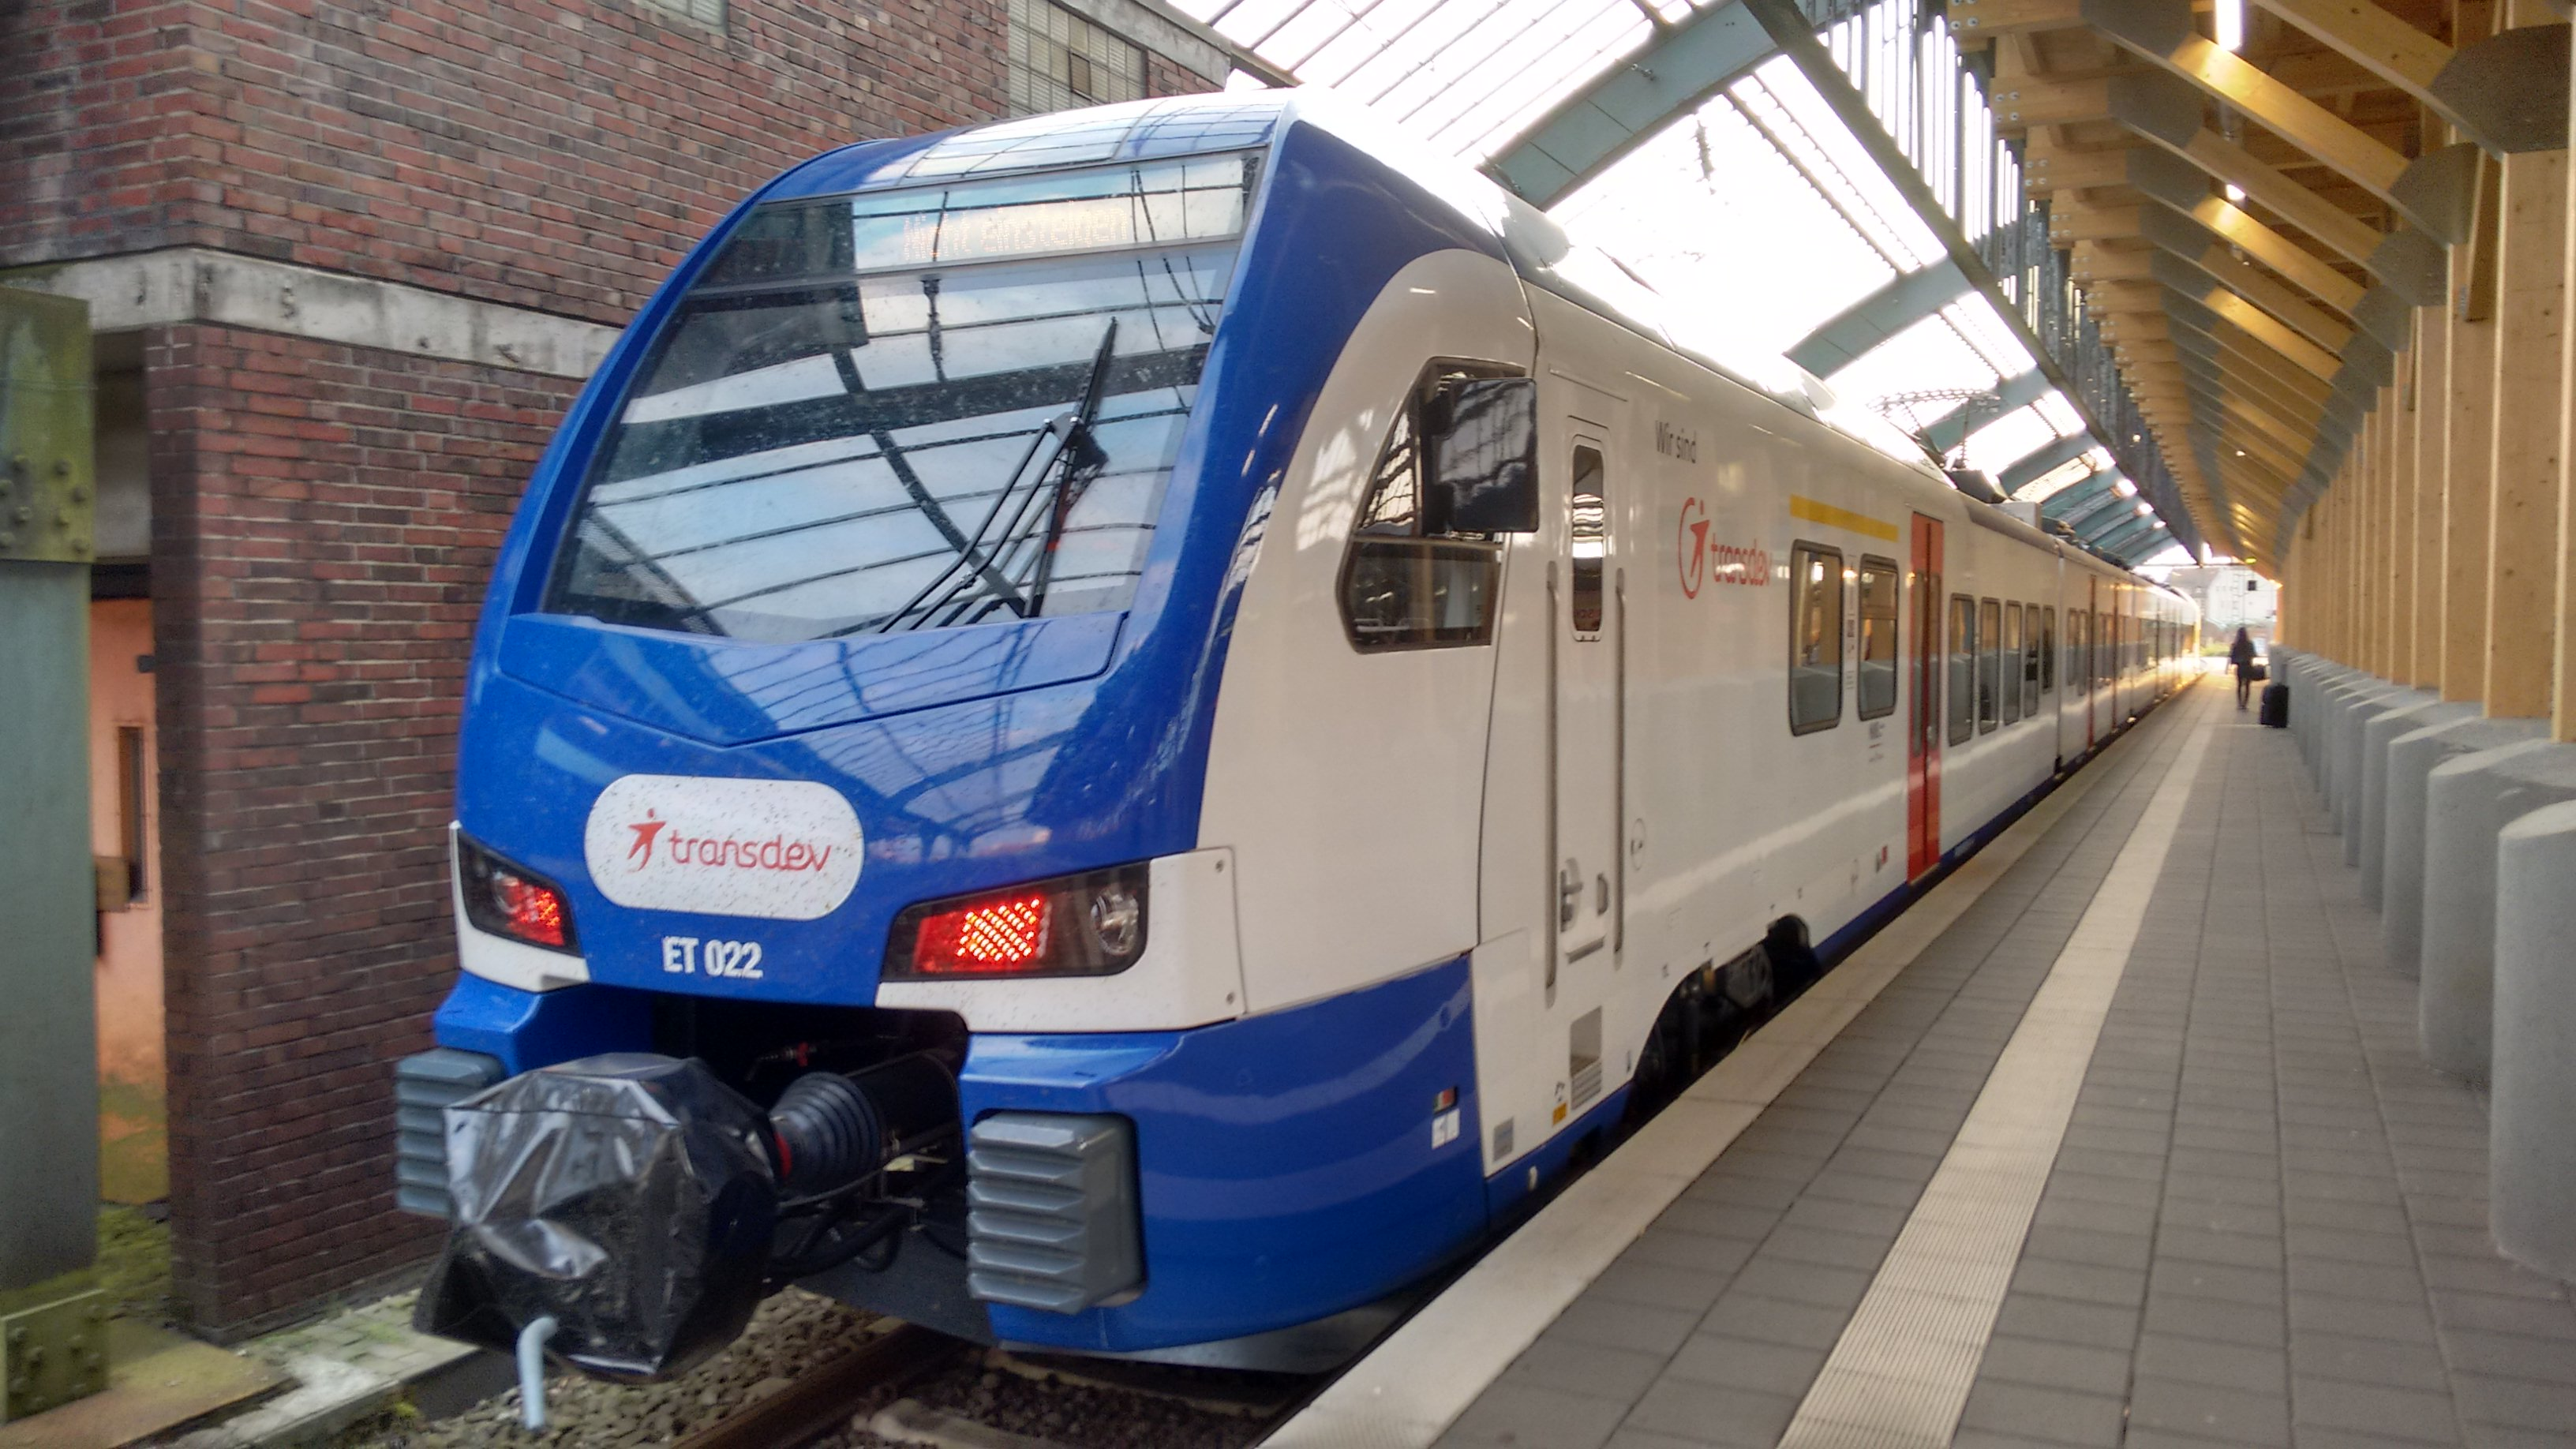
\includegraphics[width=\textwidth]{gegenwart/transdev}
			\caption{Transdev} 
		\end{subfigure}
		\begin{subfigure}{0.3\textwidth}
			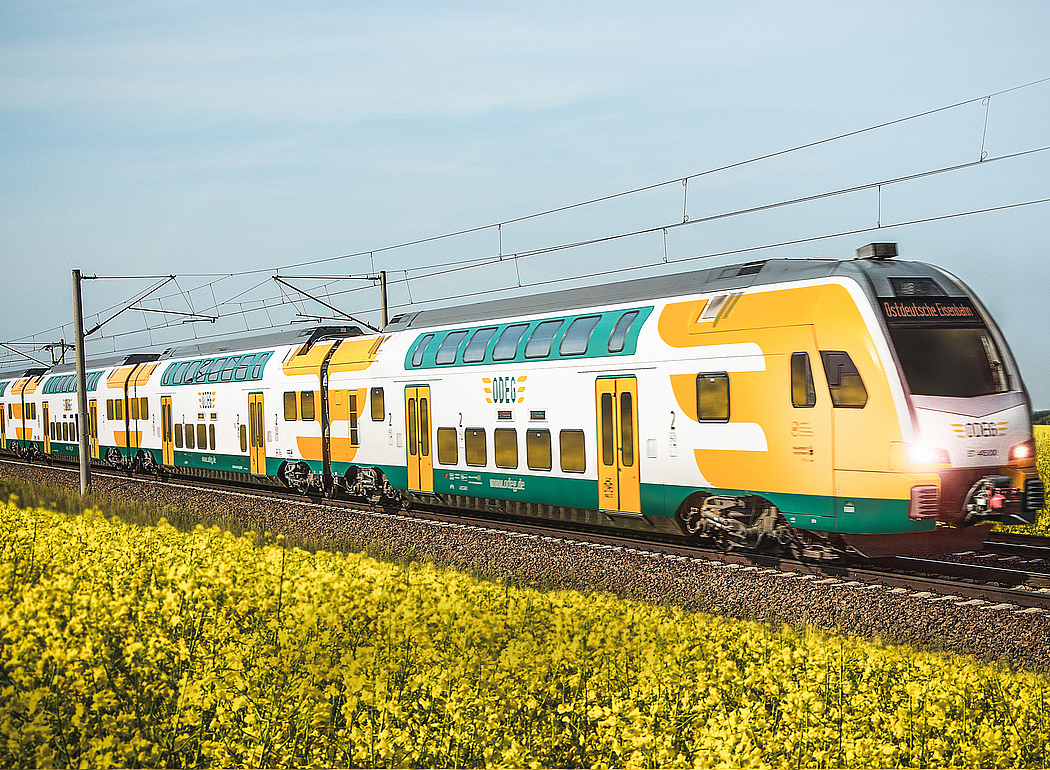
\includegraphics[width=\textwidth]{gegenwart/ODEG} 
			\caption{ODEG} 
		\end{subfigure}
	\end{figure}
\end{frame}

\subsection{Der Zustand jetzt}

\begin{frame}
\frametitle{Der Zustand jetzt}
\begin{itemize}
	\item Politik ist gut, Infrastruktur Sche**e (denk an der 49eur Ticket)
	\item Der Wettbewerb funktioniert nur fur die Regionalzugen und Guterzugen
	\item Im Thema Guterzuge hat DB Anteil verloren an der Hauptkonkurent Lkw-Verkehr an der Straße
	\item DB wird vieleicht DB Arriva oder Schenker die zwar geschulded sind aber im ganzen ein gewinnbringer sind, verkaufen
\end{itemize}
\end{frame}
\begin{frame}
\frametitle{Der Zustand jetzt}
	\centering
	\Large "Die Bahn werde ja immer subventioniert, und so toll sei die Qualität auch nicht – nee, das ist nicht so. Wenn etwas subventioniert wird, dann ist es die Straße. Aber da spricht kein Mensch drüber.“


\end{frame}
